\section{Approach}

The idea is to utilize a derivative-free optimization algorithm that iteratively selects print settings based on the user's ranking of previous test prints. Ultimately, leading towards better print settings with each iteration. The requirement for the user to rank given print settings by their outcome is the reason why the paper has the compound word "semi-automatic" in its title. The user acts as the objective function which in turn leads to no "fully automatic" optimization because user interaction is required. Objective functions, sometimes referred to as black-box functions \cite{agnihotri2020exploring, larson2019derivative}, return a numerical value based on given input parameters which is either min- or maximized. The returned value quantifies how good or bad given input parameters are \cite{rios2013derivative}. In the scope of this paper, the input parameters are the print settings and the output is the users ranking of the test print. The reason for relying on derivative-free algorithms is the fact that obtaining derivatives of the objective function with the proposed ranking approach is not possible. As the name suggests, derivative-free algorithms are suitable for optimization problems where obtaining the derivatives of the objective function is not possible or too computationally expensive \cite{rios2013derivative}. A ranking approach is chosen as opposed to a score-based approach to reduce expected noise. In simplified terms, noise describes a perceived change in the model (optimization process) although the perceived change is wrong. It is hard to impossible to quantify precisely (through a score e.g. from 1-10) how much better or worse a print's quality is by looking at the object. On the contrary, it is possible to determine and numerically express (through a ranking) if an object is of better quality, or not, than another.

\subsection{Evaluation of other Approaches}
The reason for relying on the user's judgment lays in the impossibility (to the author's knowledge) of formulating an objective function using another metric without relying on computer vision or sensors. Both computer vision and sensors did not seem feasible during the time of writing which is further elaborated below. Generally, little research regarding the optimization of print settings in the scope of personal 3D printers has been found/conducted. A possible reason for the relatively sparse research might be explained by the relative "newness" of personal 3D printers and the niche market of hobbyists currently being served by the technology \cite{sauramo2014proliferation, khan2020real}.

\subsubsection{Computer Vision}

\begin{wrapfigure}{r}{0.45\textwidth}
    \centering
    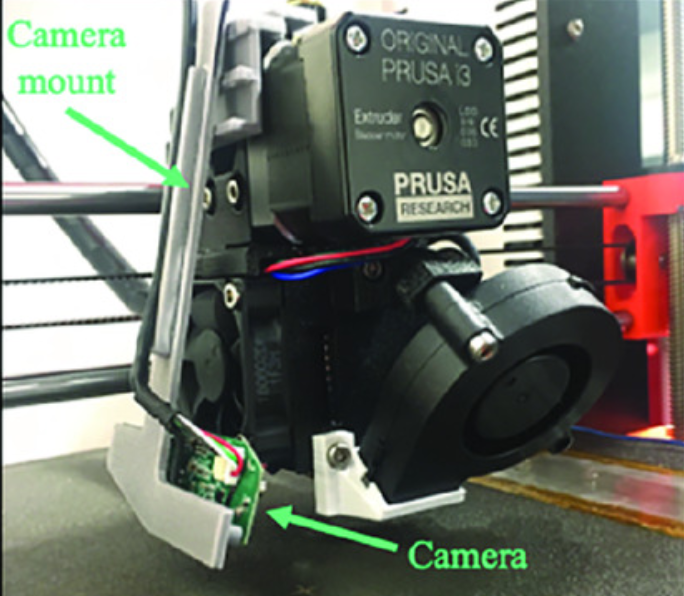
\includegraphics[width=0.9\linewidth]{assets/computer_vision_illustration.png}
    \caption{Zeqing Jin, Zhizhou Zhang, and Grace X Gu. used computer vision to train a machine learning model which can detect print defects and adjust print settings accordingly by mounting a camera on the extruder. The figure is taken from their research paper \cite{jin2019autonomous}.}
    \label{figure/mountedCamera}
\end{wrapfigure}

Initially, the utilization of computer vision was intended. A computer vision approach would enable more autonomous optimization, potentially in real-time. The idea was to mount a camera on top of the extruder, or attaching it onto the frame of the 3D printer. The camera, in combination with a classification model, would be used to detect print defects of a currently in-print object. Based on detected print defects, print settings could be adjusted accordingly. Multiple recently published papers utilized a camera to detect print defects and accomplished decent results, indicating that the general idea of utilizing a camera/computer vision is feasible in the context of classifying print defects \cite{khan2020real, paraskevoudis2020real, jin2020automated, jin2019autonomous}. One team of researchers managed to automatically adjust the print setting that influences the detected defect in real-time \cite{jin2019autonomous}, coming close to the idea of self-calibrating 3D printers, or at least a sort of automatic self-calibration. However, utilizing computer vision requires training data. Zeqing Jin et al. used 360.000 images in one of their research papers to train their models \cite{jin2019autonomous}. Jin et al. likely used data augmentation to achieve such a high number of training images \footnote{Data augmentation refers to a set of techniques that modify images in such a way that the modified images are perceived as different images by a machine learning algorithm compared to the original images \cite{perez2017effectiveness}. The result is a cheap method to artificially increase the number of images in a dataset.}, and the constant feed of images (video) during a print likely also magnified the number of training images. Nevertheless, generating a training dataset requires lots of prints which is time-intensive. Paraskevoudis et al. developed a classification model with as few as 500 un-augmented images which can detect stringing, see figure \ref{figure/stringing} for an example of stringing \cite{paraskevoudis2020real}. But even generating 500 images was determined as too time-consuming for this project. The smallest test prints take at least 5-10 Minutes, more like 15-20 Minutes, and only test one or two very specific settings.

As promising as a computer vision approach is, the required amount of training data is too resource-intensive to obtain and ultimately led to the decision to not utilize computer vision.


\subsubsection{Sensors}
Leveraging sensors which could act as an objective metric, or be used in a machine learning approach, did not seem promising at the time of writing. Currently, personal FDM 3D printers have a very sparse amount of sensors. The list includes the "position" of the stepper motors (X,Y,Z and the filament motor E), the extruder's temperature (print temperature), print bed temperature (surface temperature) and fan speed. The print settings themselves are handled by slicing software. Slicing software converts 3D models into printable g-code. G-code is a numerical control language for manufacturing machines that has been adopted by the RepRap project and is used by the majority, if not all, personal 3D printers \cite{gcodeRepRap}. The RepRap project was a research initiative to develop an open-source 3D printer that can print (replicate) itself and acted as "root" design for most low-cost personal 3D printers \cite{jones2011reprap}. Figure \ref{figure/gcode_example} (b) shows a g-code file containing instructions which results in the print of a 10mm x 10mm rectangle as illustrated to the left in figure \ref{figure/gcode_example} (a).

Simplified, g-code is just an instruction set that instructs the manufacturing machine, i.e. the 3D printer, to move the step motors X,Y,Z and the filament motor called E in a specific direction. Moving the axis X, Y, Z axis and simultaneously moving i.e. "pushing" or "retracting" filament with E leads to the printing of an object. In its simplicity lays the reason for the lack of sensors of 3D printers and why the g-code generation (slicing) is of more importance than the g-code itself. Different 3D printers printing the same g-code does not lead to the same print quality among all printers. Each 3D printer, and even filament, can require different print settings which are handled by the slicing software. It follows that the purpose of slicing software is not only the transformation of 3D models into g-code but generating "custom" g-code given a 3D model and a set of print settings. 

In conclusion, using the printers step motor sensors X, Y, Z and E in combination with the g-code which would act as objective/truth-value did not seem promising because the printer prints the g-code correctly in most cases; but the g-code itself has not been optimized for the specific printer.


\subsubsection{Guided Local Search}

The first developed approach to algorithmically optimize 3D print settings in the context of this paper was a local search algorithm inspired by current state-of-the-art manual optimization of retraction settings \cite{teachingTechCalibration}. Retraction settings determine how much filament is "retracted" just before the print head moves to another point without extruding plastic on its way. If the retraction is too low, stringing can occur. If the retraction is too high, gaps in the surface can occur. An illustration of stringing is shown in figure \ref{figure/stringing}. 
The user was required to print a tower-like object which was split into different segments. Each segment was printed with different retraction settings whereas the set of all segments act as the range of a specific setting. After each print, the user was prompted to define the two best segments. The algorithm then returned a new test object whereas the print settings of each segment lay within the range of the previous two best segments. Figure \ref{figure/local_search_illustration} illustrates one iteration with further explanation. 

The approach replicated manual optimization more algorithmically. Thus, it inherited the same shortcoming: Simultaneous multivariable optimization is not possible or takes too many iterations which is crucial considering the print time and manual labor required for each iteration. Simultaneous refers to optimizing multiple variables at once instead of optimizing "one variable after another". Because of the lack of simultaneous multivariable optimization, the approach was not further developed but might offer value to users due to the more algorithmic "manual" optimization. 

\begin{figure}[h]
    \centering
    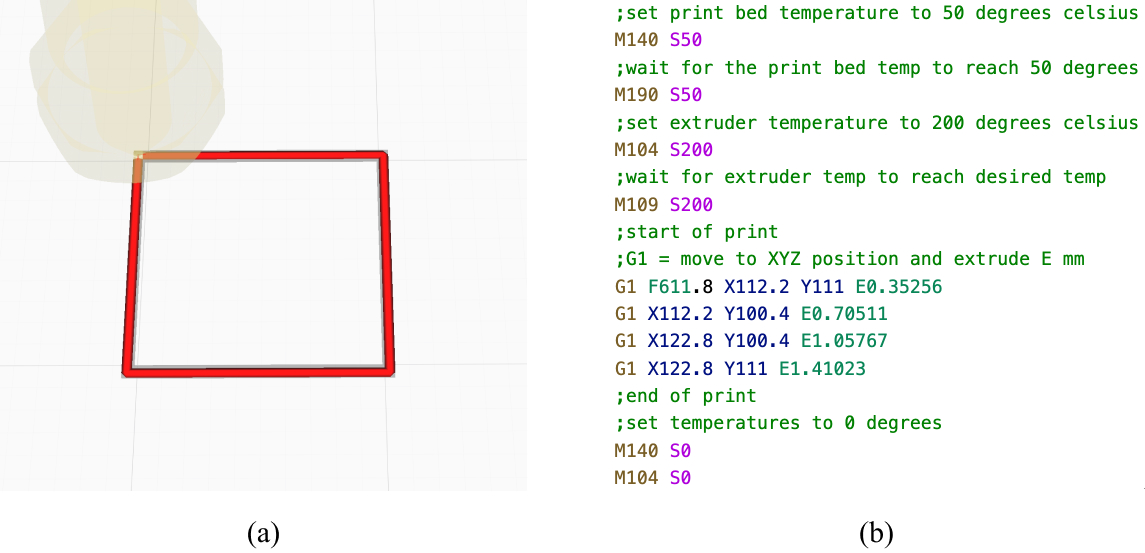
\includegraphics[width=0.75\linewidth]{assets/model_gcode_example.jpg}
    \caption{Exemplary 3D model on the left (a) and corresponding g-code on the right (b). Each line in the g-code on the right is an instruction. Instructions beginning with M regard the temperature of the print bed or extruder. The G1 instructions are the actual print of the object and contain the instruction to move X, Y, Z and the extruder/filament motor E. The model can thus be printed in four movement steps G1.}
    \label{figure/gcode_example}
\end{figure}

\begin{figure}[!b]
  \centering
  \begin{minipage}[b]{0.4\textwidth}
    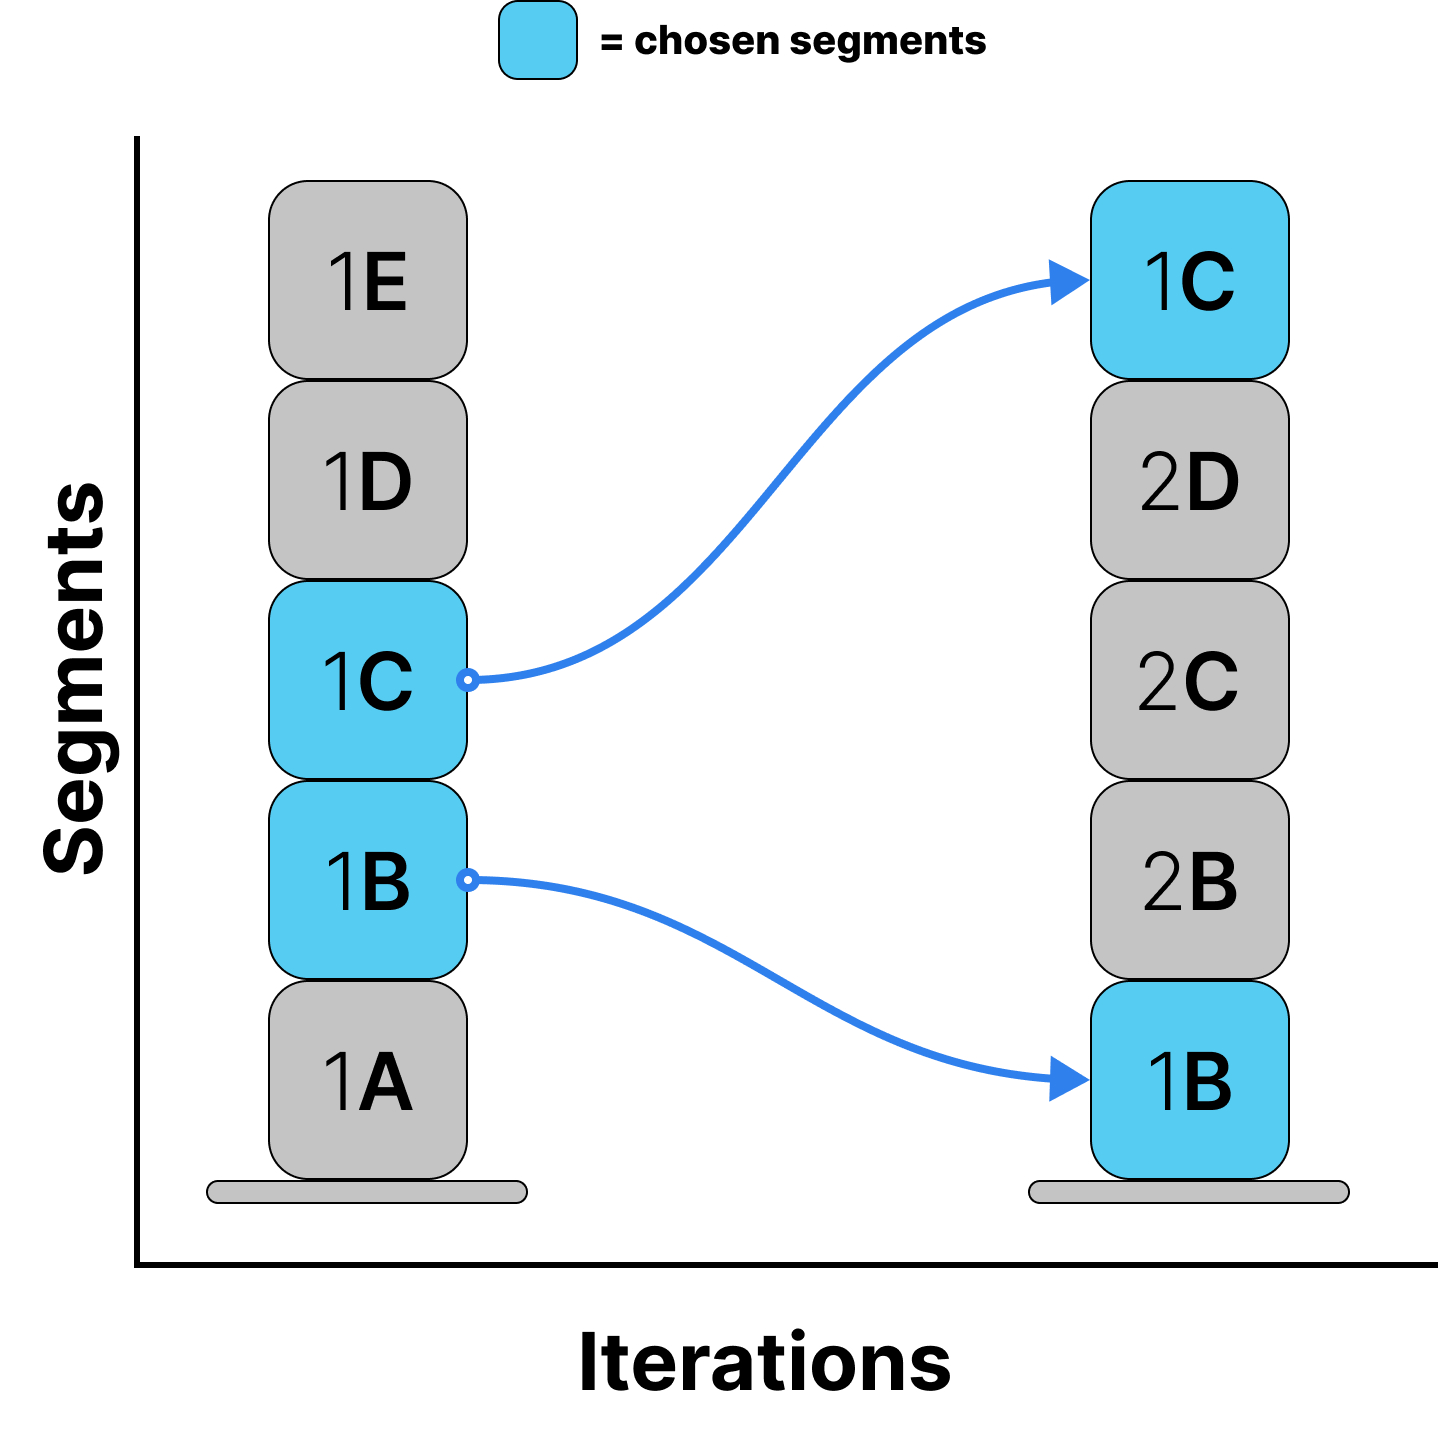
\includegraphics[width=\textwidth]{assets/local_search_illustration.jpg}
    \caption{Illustration of the Guided Local Search approach showing one iteration. For example, the segments 1A to 1E form a range over a print setting e.g. 180\textdegree C to 230\textdegree C in 10\textdegree C steps. 1B and 1C have been chosen as the best segments. Then next iteration forms segments ranging from 1B to 1C. Resulting in a range from 190\textdegree C to 200\textdegree C in 2\textdegree C steps.}
    \label{figure/local_search_illustration}
  \end{minipage}
  \hfill
  \begin{minipage}[b]{0.45\textwidth}
    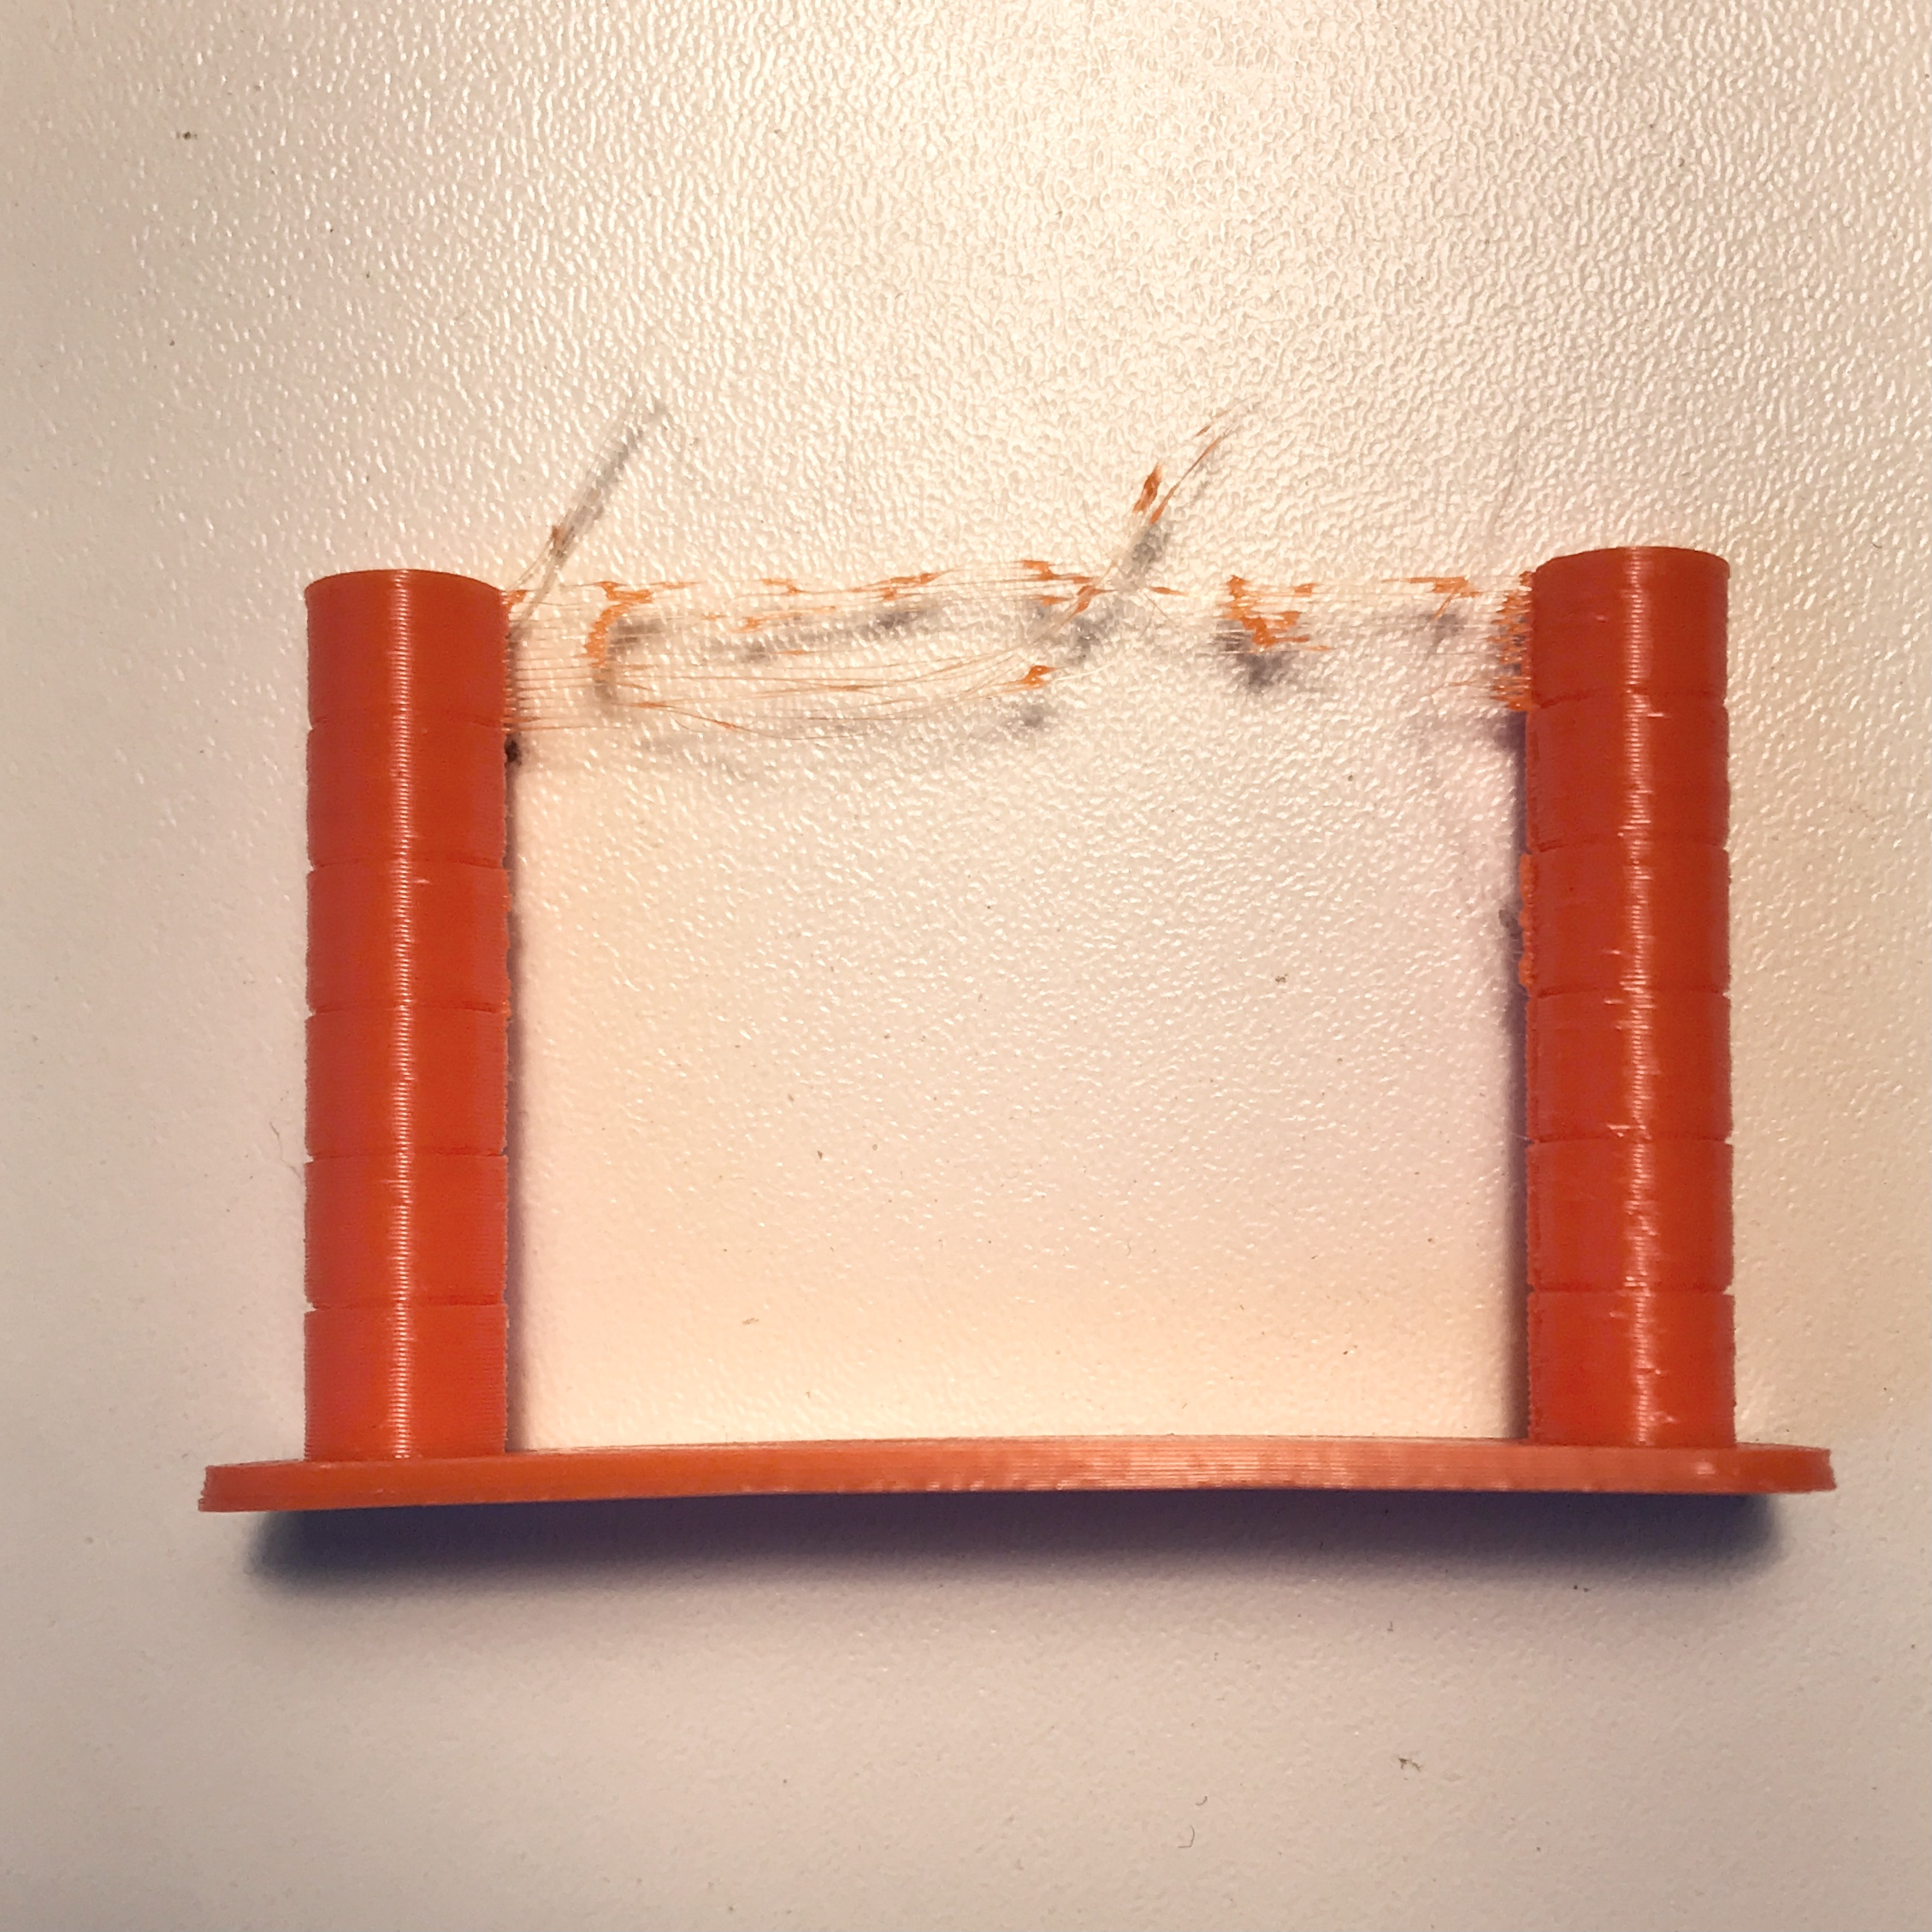
\includegraphics[width=\textwidth]{assets/stringing.jpg}
    \caption{A typical stringing test object which has stringing in the upper part of the object. Stringing can occur if the retraction distance is not optimal. Each time the print head "travels" from one point to another, plastic must not be extruded. However, not extruding plastic is not enough. The plastic needs to be retracted from the nozzle right before starting the start of the "travel" and pushed back into the nozzle once arrived. If the retraction distance is too low, the plastic in the nozzle keeps "sticking" to the object. When the print head now starts moving, the sticking plastic creates strings. Similar to melted cheese on a pizza.}
    \label{figure/stringing}
  \end{minipage}
\end{figure}

% \begin{figure}[h]
%     \centering
%     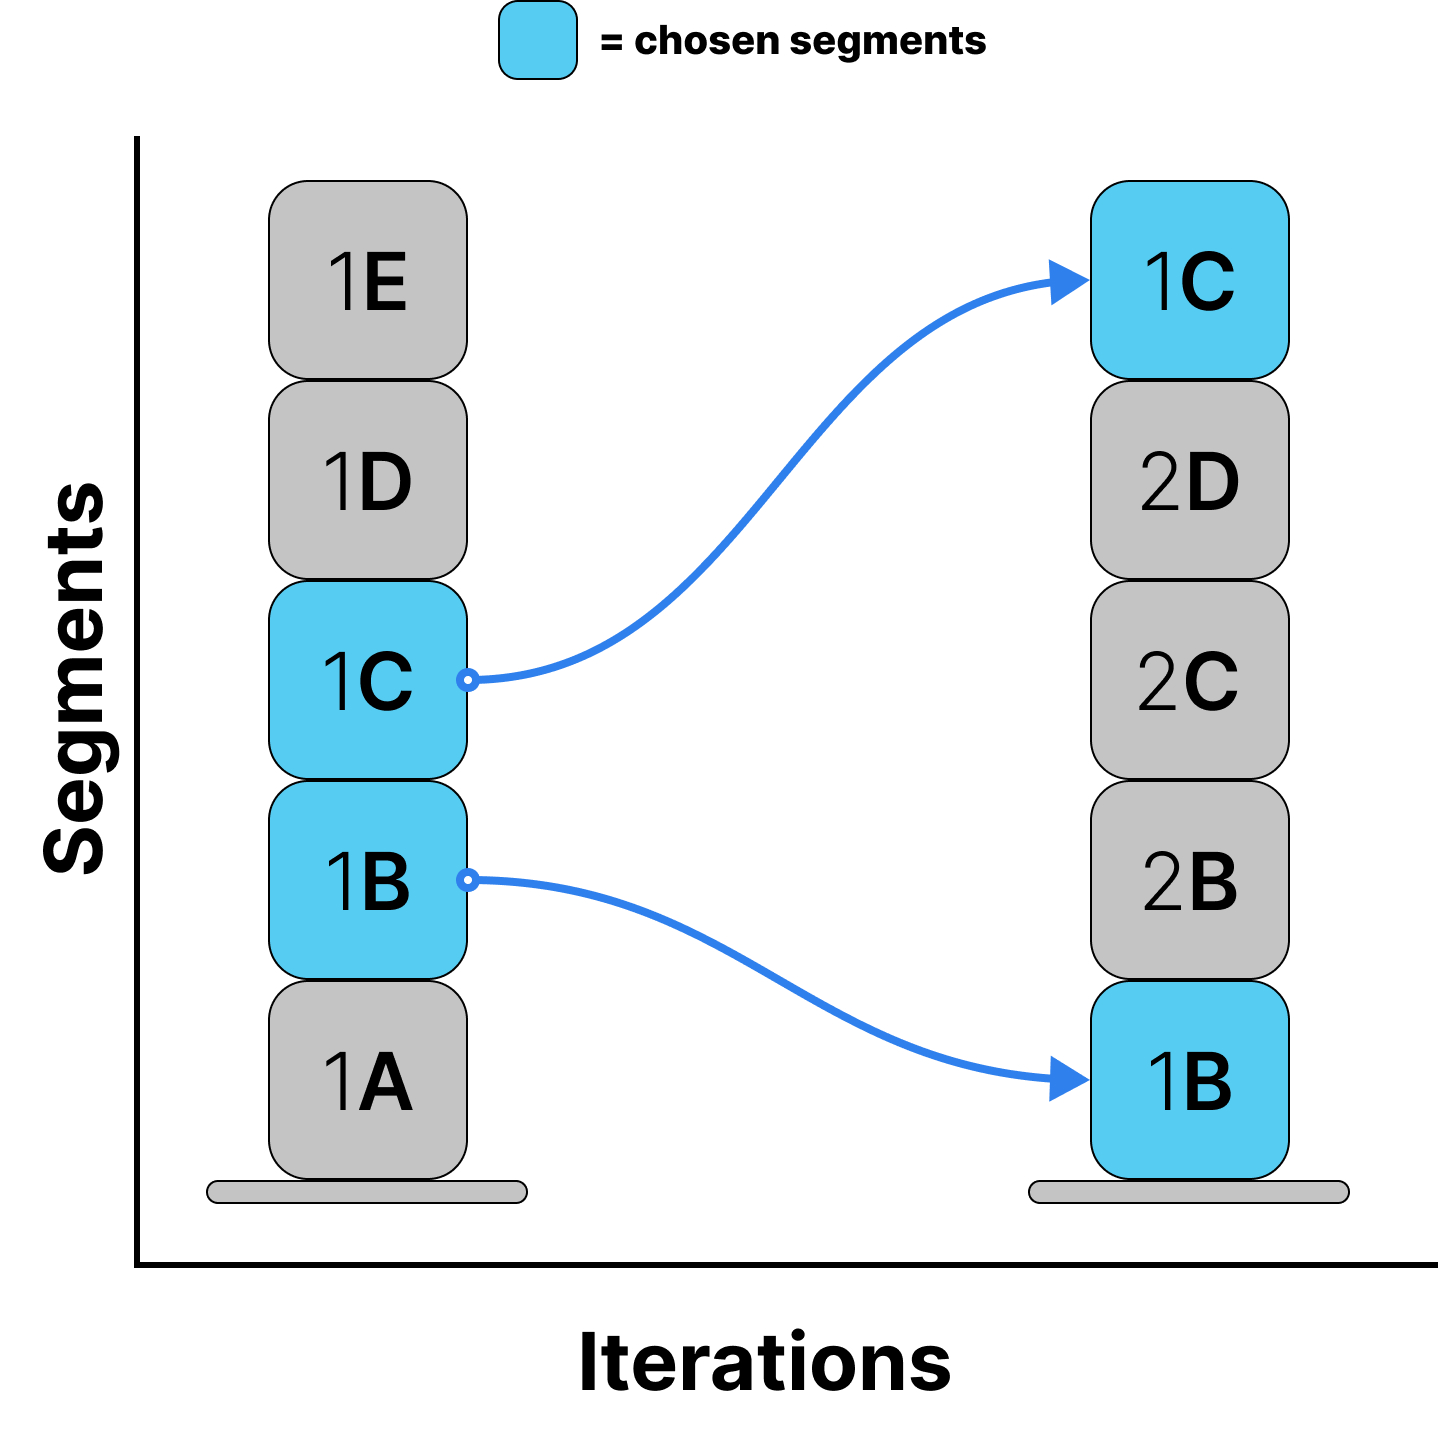
\includegraphics[width=0.35\linewidth]{assets/local_search_illustration.jpg}
%     \caption{Illustration of the Guided Local Search approach showing one iteration. For example, the segments 1A to 1E form a range over a print setting e.g. 180 degrees to 230 degrees in 10 degree steps. 1B and 1C have been chosen as the best segments. Then next iteration forms segments ranging from 1B to 1C. Resulting in a range from 190 degrees to 200 degrees in 2 degree steps.}
%     \label{figure/local_search_illustration}
% \end{figure}


% \begin{figure}[h]
%     \centering
%     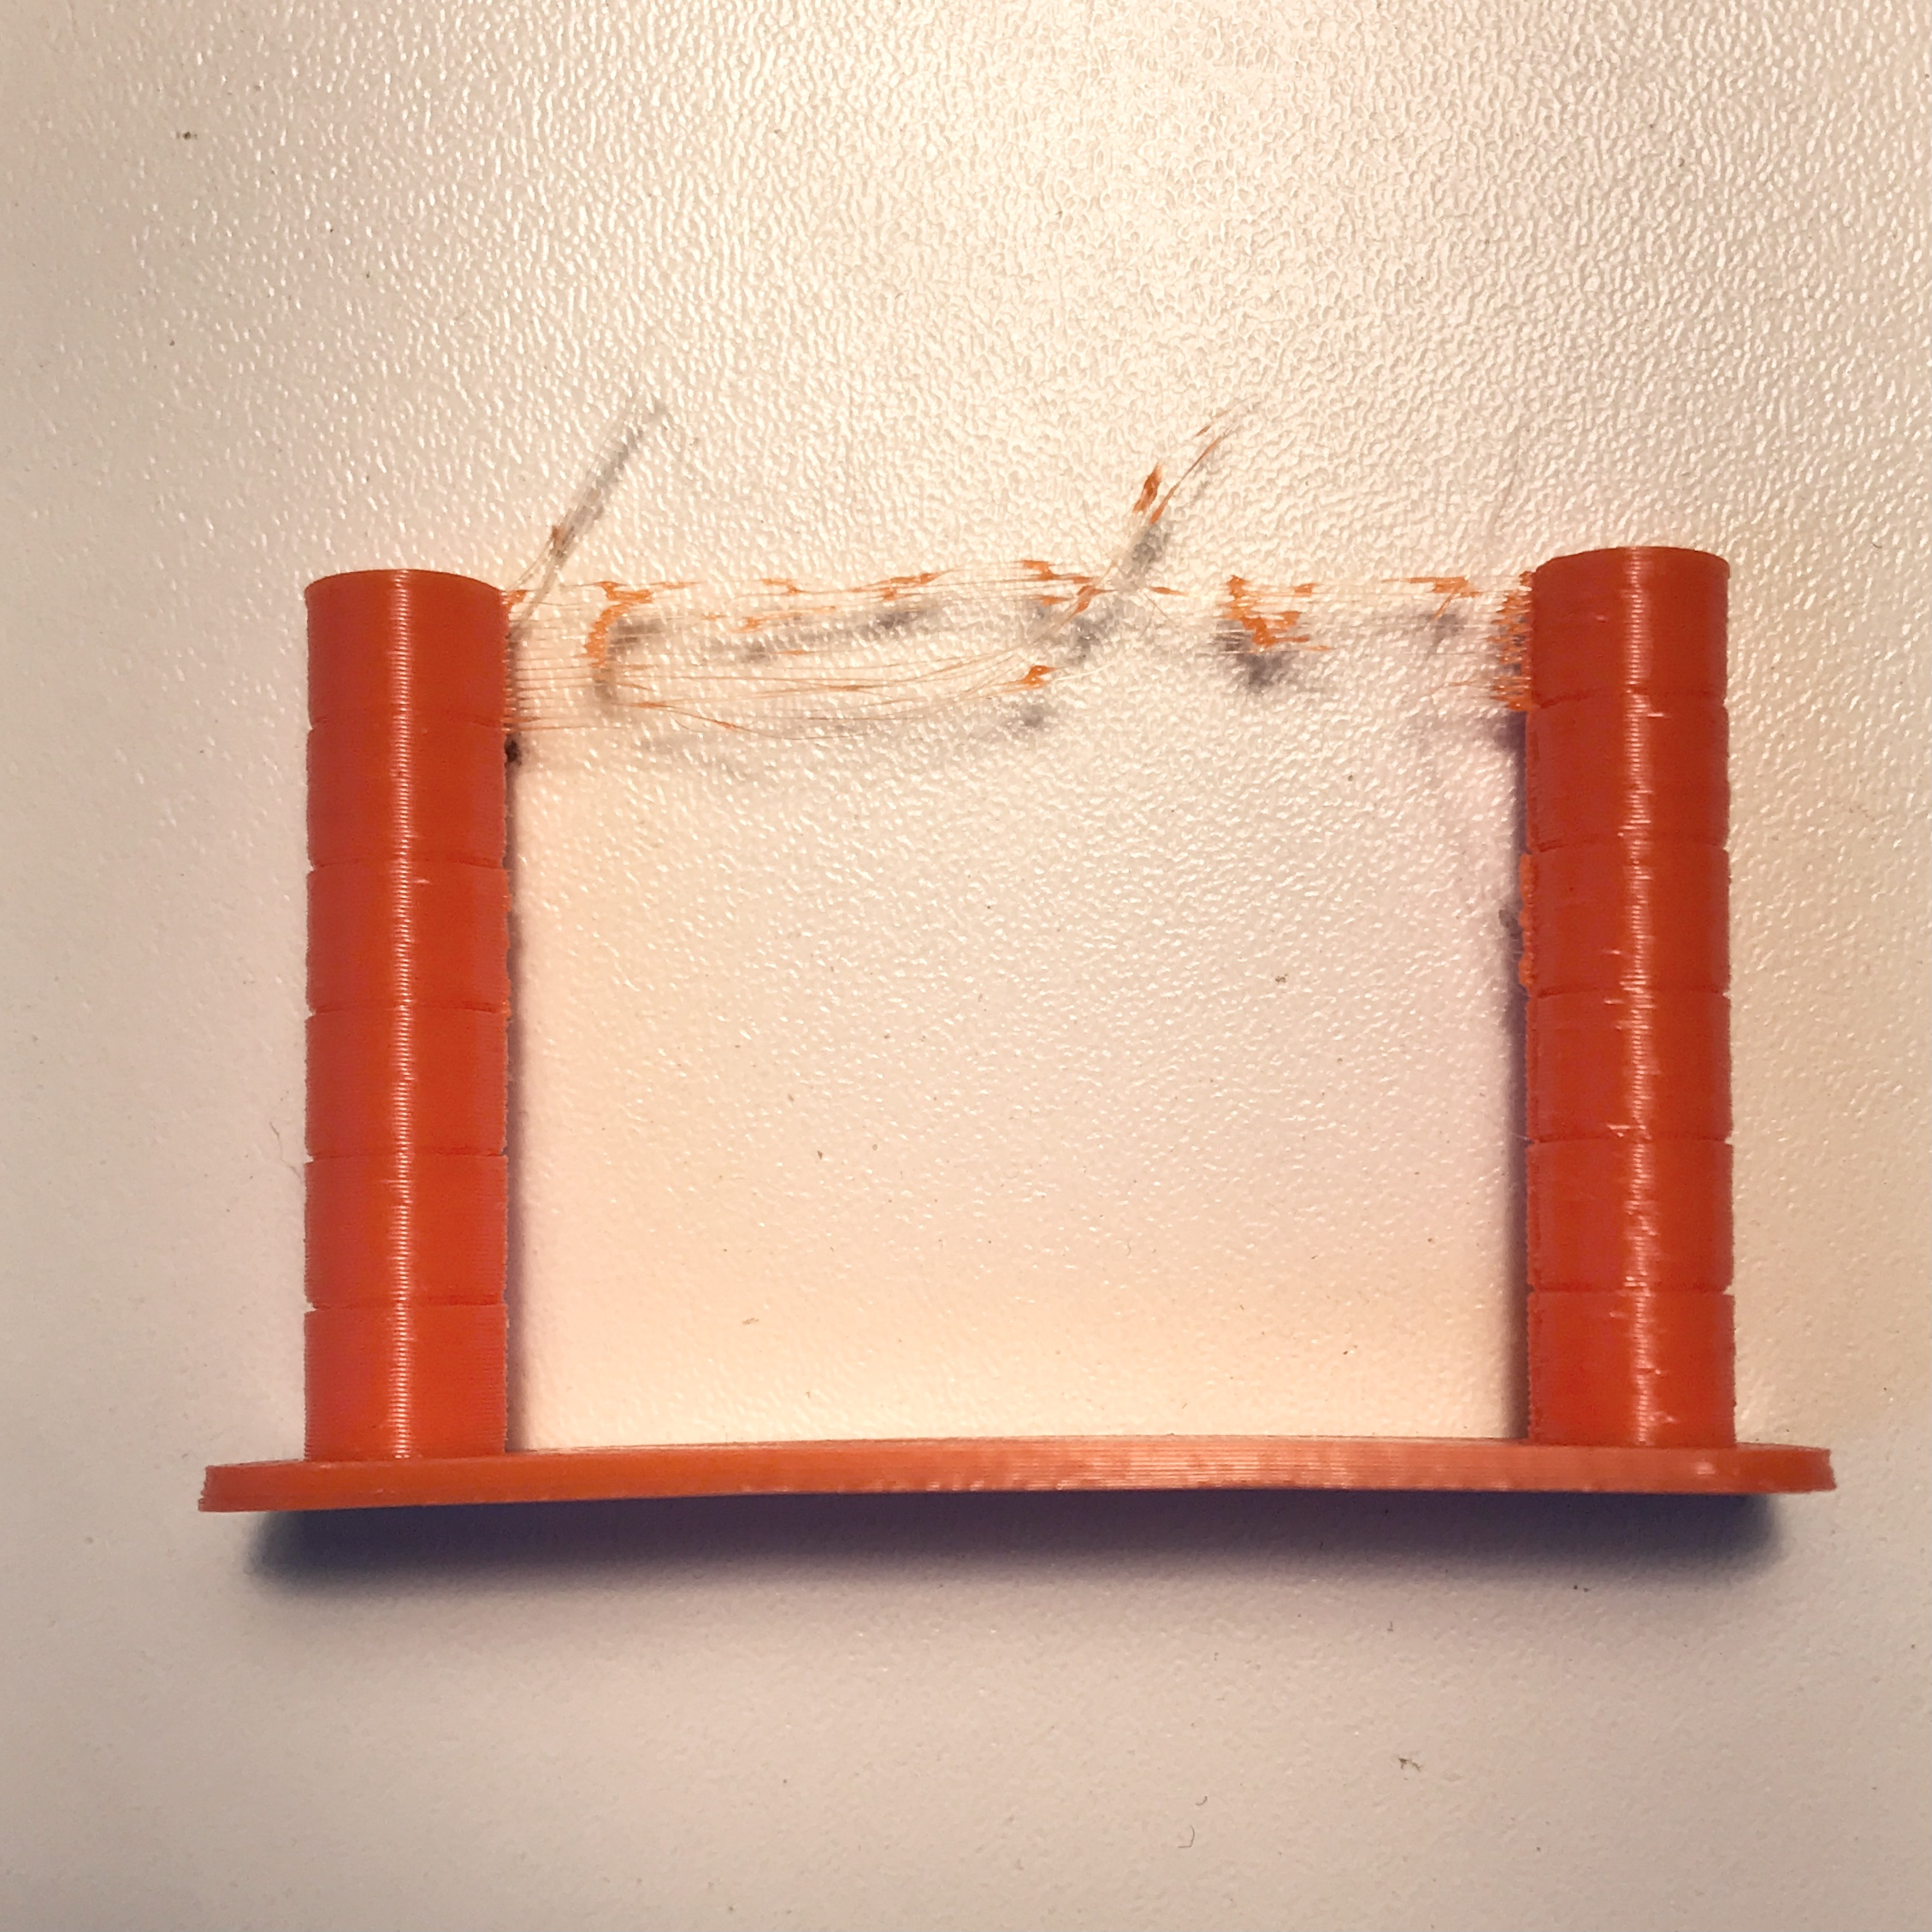
\includegraphics[width=0.3\linewidth]{assets/stringing.jpg}
%     \caption{The figure shows a typical stringing test object which has stringing in the upper part of the object. Stringing can occur if the retraction distance is not optimal. Each time the print head "travels" from one point to another, no plastic must be extruded. Just stopping to extrude plastic right before starting to "travel" is not enough. The plastic needs to be retracted from the nozzle right before starting to travel and pushed back into the nozzle once arrived. If the retraction distance is too low, the plastic in the nozzle keeps "sticking" to the object. When the print head now starts moving, the sticking plastic creates strings. Similar to melted cheese on a pizza.}
%     \label{stringing}
% \end{figure}
